\documentclass[11pt,a4paper]{article}
\usepackage[margin=25mm]{geometry}
\usepackage{fontspec,unicode-math,booktabs,graphicx,hyperref}
\setmainfont{STIXGeneral}\setmathfont{STIX Two Math}\hypersetup{hidelinks}
\setlength{\emergencystretch}{2em}
\title{Coset geometries and symmetric group markings: unified proof costs}
\author{Human Compression project}\date{Numerical candidate awaiting independent review}
\begin{document}\maketitle
The complete written comparison for the five fixed original texts is
\[
 \frac{\sum_i c(L_i)}{c(U_B)+\sum_i c(B_i)}
 =\frac{124,906}{44,905+69,265}
 =\frac{124,906}{114,170}=\mathbf{1.094035}.
\]
The numerator keeps the accepted source representations: N001's complete literal authored-browser rendering and the four complete PDFs. N001's original PDF remains unavailable; no complete-PDF factor for all five originals is claimed. The L040 identification cover remains in the primary input.

The entire sixteen-page common paper is charged once. It replaces the two earlier common papers through reviewed mathematical arguments, and all five complete applications remain. The fifty-page current input bundle includes references and the seven-page complete program appendix.

\begin{center}\begin{tabular}{lrrr}\toprule
Matched original & Original & Application & Conditional\\\midrule
N001: Inductively minimal geometries & 14,519 & 7,371 & 1.969746\\
N003: Maximal symmetric markings & 17,780 & 9,155 & 1.942108\\
N008: Frattini coordinate geometries & 18,009 & 11,132 & 1.617769\\
L030: Disjoint-subset geometries & 22,704 & 12,286 & 1.847957\\
L040: High-rank symmetric markings & 51,894 & 29,321 & 1.769858\\
\bottomrule\end{tabular}\end{center}
Every conditional factor presupposes acquisition of the \emph{whole current common theory and all four complete declared programs}. Each local paper, including context and references, is then charged in full. The common cost is 44,905 characters.

\begin{center}\begin{tabular}{lrr}\toprule
Complete-topic boundary & Denominator & Factor\\\midrule
Written common and all five applications &114,170&1.094035\\
Also the entire printed program appendix &127,340&0.980886\\
Also the four whole raw programs (alternative) &126,500&0.987399\\\bottomrule
\end{tabular}\end{center}
The appendix costs 13,170 characters; the raw files cost 12,330. These are alternative representations, never additive charges. One program supplies bounded primitive-group inputs, two validate written general arguments, and one supplies the separate degree-eight example and branching-presentation check. No program is pruned because its role is auxiliary.

Two current operational drivers (15,442 characters) and two Lean files (8,377 characters) are separately inventoried. The fourteen reused declarations remain partial formal evidence. Full external proof, graphical and historical software costs remain unknown, not zero. No source, question or formal credit changes.
\newpage
\section*{Whole theory and complete applications}
\begin{center}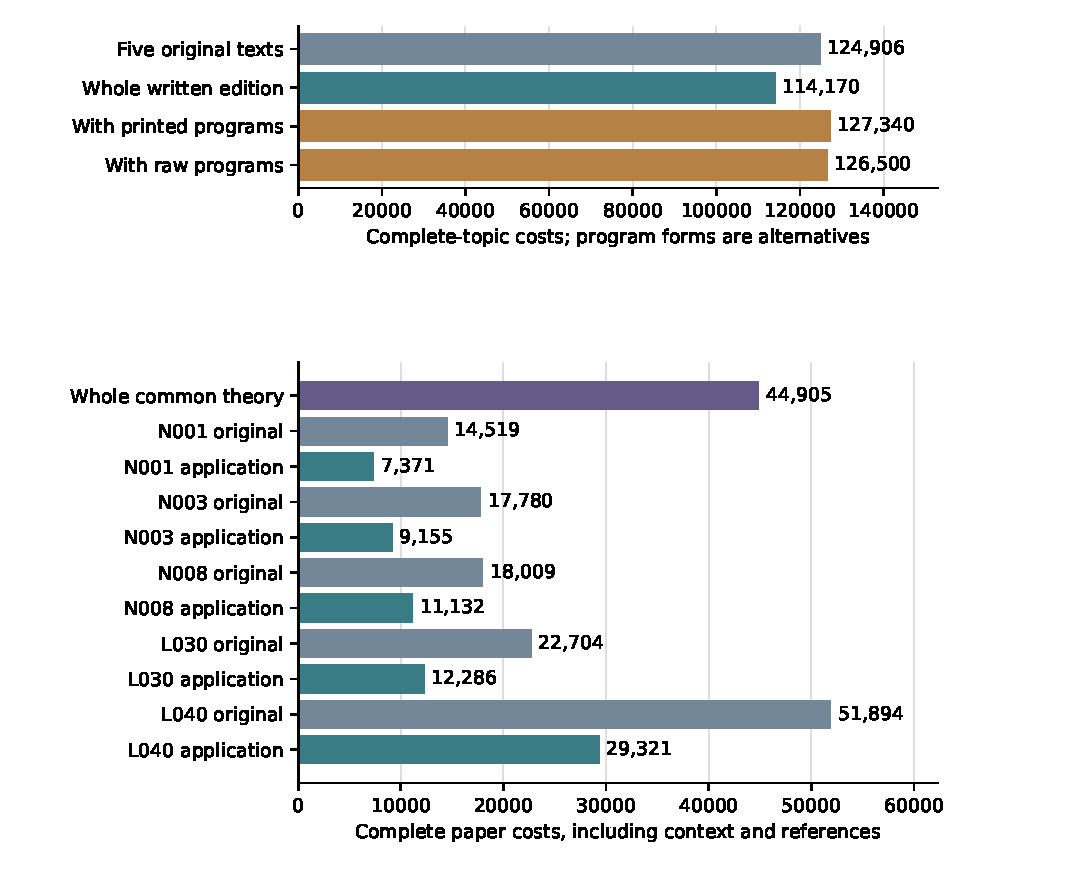
\includegraphics[width=\linewidth]{costs.pdf}\end{center}
The lower bars compare full paper costs. Their conditional ratios require the common theory and complete programs already to have been acquired. The current written denominator pays the common paper once; it does not omit it or add both prior common papers.

\begin{center}\begin{tabular}{lrrr}\toprule
NFC nonspace sensitivity & Original total & Written total & Factor\\\midrule
Complete raw text (primary) & 124,906 & 114,170 & 1.094035\\
Selected literal text & 123,210 & 114,118 & 1.079672\\
Selected calibrated text & 123,210 & 114,118 & 1.079672\\
L040 article-only, otherwise primary & 124,125 & 114,170 & 1.087195\\
\bottomrule\end{tabular}\end{center}
The primary counts raw, untrimmed NFC nonspace characters. All thirty settings---three extraction conventions, two normalizations and five units---are retained. The separate direct L040 article-only input changes only that source cost; all replacement costs and the other four conditionals stay unchanged. Complete JSON and CSV records give 240 main exact fractions and 120 cover-sensitivity fractions.

The earlier numerical edition is preserved. These results reuse the independently accepted inputs; no source extraction, font calibration, GAP or Lean is rerun here. The numerical author also authored those inputs, which received distinct root acceptance. This numerical candidate still requires its own independent review.
\end{document}
